\documentclass{../../../oss-ap12ibhl-print}

\begin{document}
\genheader

\gentitle{4}{MOMENTUM, IMPULSE AND COLLISIONS}

\begin{questions}

  \question A toy train car of mass \SI3{\kilo\gram} rolls to the left at
  \SI2{\metre\per\second} and collides with a \SI4{\kilo\gram} train car
  rolling to the right at \SI1{\metre\per\second}. The two cars stick together.
  The velocity of the cars after the collision is
  \begin{choices}
    \choice $2/7$ \si{\metre\per\second} to the left
    \choice $2/7$ \si{\metre\per\second} to the right
    \choice $4/7$ \si{\metre\per\second} to the left
    \choice $4/7$ \si{\metre\per\second} to the right
    \choice $9/7$ \si{\metre\per\second} to the right
  \end{choices}

  \uplevel{
    \textbf{Questions \ref{impulse1}--\ref{impulse2}}. A force acts on a
    \SI{2.}{\kilo\gram} mass during a time interval as shown in the graph.
    \begin{center}
      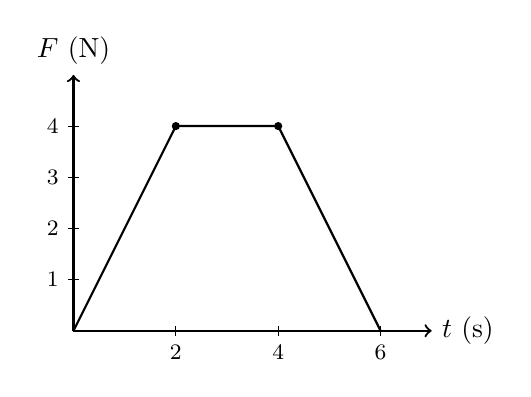
\begin{tikzpicture}[scale=.65]
        \draw[thick,->](0,0)--(7,0) node[right]{$t$ (s)};
        \foreach \y in {1,...,4}{
          \draw(-.1,\y)--(.1,\y) node[pos=0,left]{\footnotesize\y};
        }
        \draw[thick,->](0,0)--(0,5) node[above]{$F$ (N)};
        \foreach \x in {2,4,6}{
          \draw(\x,-.1)--(\x,.1) node[pos=0,below]{\footnotesize\x};
        }
        \draw[thick](0,0)--(2,4)--(4,4)--(6,0);
        \fill(2,4) circle(.08);
        \fill(4,4) circle(.08);
      \end{tikzpicture}
    \end{center}
  }

  \question The impulse given to the mass from $t=0$ to $t=\SI6{\second}$ is
  \label{impulse1}
  \begin{choices}
    \choice\SI4{\newton\second}
    \choice\SI8{\newton\second}
    \choice\SI{12}{\newton\second}
    \choice\SI{16}{\newton\second}
    \choice\SI{24}{\newton\second}
  \end{choices}
    
  \question If the initial speed of the mass is \SI2{\metre\per\second} at
  $t=0$, what is its speed at the end of 6 s?
  \label{impulse2}
  \begin{choices}
    \choice\SI4{\metre\per\second}
    \choice\SI6{\metre\per\second}
    \choice\SI8{\metre\per\second}
    \choice\SI{10}{\metre\per\second}
    \choice\SI{16}{\metre\per\second}
  \end{choices}
    
  \question Two steel balls, one of mass $m$ and the other of mass $2m$,
  collide and rebound in a perfectly elastic collision. Which of the following
  is conserved in this elastic collision?
  \begin{choices}
    \choice velocity only
    \choice momentum only
    \choice momentum and kinetic energy only
    \choice momentum, velocity, and kinetic energy
    \choice kinetic energy only
  \end{choices}
  \newpage
  
  \question Two blocks are connected by a compressed spring and rest on a
  frictionless surface. The blocks are released from rest and pushed apart by
  the compressed spring. If one mass is twice the mass of the other, which of
  the following is the same for both blocks?
  \begin{choices}
    \choice magnitude of momentum
    \choice acceleration
    \choice speed
    \choice kinetic energy
    \choice potential energy
  \end{choices}

  \question A \SI{1000}{\kilo\gram} railroad car is rolling without friction on
  a horizontal track at a speed of \SI{3.}{\metre\per\second}. Sand is poured
  into the open top of the car for a time of \SI{5.}{\second}. The speed of
  the car after \SI{5.}{\second} is \SI{1.}{\metre\per\second}. The mass of
  the sand added to the car at the end of \SI{5.}{\second} is

  \begin{minipage}{.4\linewidth}
    \pic{.8}{railroad-car-sand}
  \end{minipage}
  \begin{minipage}{.4\linewidth}
    \begin{choices}
      \choice\SI{500 }{\kilo\gram}
      \choice\SI{1000}{\kilo\gram}
      \choice\SI{2000}{\kilo\gram}
      \choice\SI{3000}{\kilo\gram}
      \choice\SI{3500}{\kilo\gram}
    \end{choices}
  \end{minipage}
  
  \question Two billiard balls are rolling to the right on a table as shown. The
  \SI{.4}{\kilo\gram} ball is moving faster than the \SI{.2}{\kilo\gram} ball,
  so it catches up and strikes it from behind at a slight angle. Immediately
  after the collision, the $y$-component of the \SI{.4}{\kilo\gram} ball is
  \SI{2}{\metre\per\second} downward. The $y$-component of the velocity of the
  \SI{.2}{\kilo\gram} ball must be

  \begin{minipage}{.4\linewidth}
    \begin{tikzpicture}[scale=.5]
      \draw[dashed](-3,0)--(4,0) node[right]{\small$x$};
      \draw[dashed](0,-2)--(0,4) node[above]{\small$y$};
      \draw(.3,.3) circle(.3) node[above]{\small\;\;\;\SI{.2}{\kilo\gram}};
      \draw[->](.6,.3)--(1.6,.3) node[right]{\small$v_2$};
      \draw(-2.3,-.5) circle(.5) node[below left]{\small\SI{.4}{kg}\;\;};
      \draw[->](-1.8,-.5)--(-1,-.5) node[right]{\small$v_1$};
      \end{tikzpicture}
  \end{minipage}
  \begin{minipage}{.4\linewidth}
    \begin{choices}
      \choice \SI{1}{\metre\per\second} upward
      \choice \SI{2}{\metre\per\second} upward
      \choice \SI{1}{\metre\per\second} downward
      \choice \SI{2}{\metre\per\second} downward
    \choice \SI{4}{\metre\per\second} upward
    \end{choices}
  \end{minipage}
  
  \question A \SI{.3}{\kilo\gram} baseball at rest on a tee is struck by a bat.
  The ball leaves the at with a speed of \SI{20}{\metre\per\second} at an angle
  of \ang{45} above the horizontal. The magnitude of the impulse imparted to
  the baseball by the bat is most nearly
  \begin{choices}
    \choice\SI{2}{\newton\second}
    \choice\SI{6}{\newton\second}
    \choice\SI{12}{\newton\second}
    \choice\SI{16}{\newton\second}
    \choice\SI{20}{\newton\second}
  \end{choices}

  \question Two ice skaters, a large man and a small woman, are initially at
  rest and holding each other's hands. They push away horizontally. Afterward,
  which of the following statements is true?
  \begin{choices}
    \choice They have equal and opposite kinetic energies.
    \choice The have equal and opposite momenta.
    \choice The large man applies a greater force to the small woman.
    \choice The small woman applies a greater force to the large man.
    \choice They recoil with equal and opposite velocities.
  \end{choices}

  \question A known net force $F$ acts on an unknown mass for a known time
  $\Delta t$. From this information, you could determine the
  \begin{choices}
    \choice change in kinetic energy of the object
    \choice change in velocity of the object
    \choice acceleration of the object
    \choice mass of the object
    \choice change in momentum of the object
  \end{choices}

  \uplevel{
    \textbf{Questions \ref{explode1}--\ref{explode2}}. An object has a mass
    $4m$. The object explodes into three pieces of mass $m$, $m$, and $2m$. The
    two pieces of mass $m$ move off at right angles to each other with the same
    momentum $mv$, as shown.
    \begin{center}
      \begin{tikzpicture}[scale=.6]
        \draw[thick,dashed](-1.5,0)--(3,0);
        \draw[thick,dashed](0,-1.5)--(0,3);
        \draw[thick](0,0) circle(.5);
        \fill[thick](-1.5,0) circle(.15) node[above]{\small $m$};
        \fill[thick](0,-1.5) circle(.15) node[right]{\small $m$};
        \draw[very thick,->](-1.5,0)--(-3,0)node[left]{\small$mv$};
        \draw[very thick,->](0,-1.5)--(0,-3)node[below]{\small$mv$};
      \end{tikzpicture}
    \end{center}
  }

  \question The speed of mass $2m$ after the explosion is
  \label{explode1}
  \begin{choices}
    \choice $2v$
    \choice $\displaystyle\sqrt2v$
    \choice $\dfrac{\sqrt2}2v$
    \choice $\dfrac{\sqrt2}3v$
    \choice $\dfrac{\sqrt3}2v$
  \end{choices}
  
  \question The direction of velocity of mass $2m$ is
  \label{explode2}
  \begin{choices}
    \choice $\rightarrow$
    \choice $\swarrow$
    \choice $\downarrow$
    \choice $\nearrow$
    \choice $\uparrow$
  \end{choices}
  
  \question A block of mass $m$ is moving to the right with a speed $v_0$ on a
  horizontal surface of negligible friction when it explodes. The explosion
  causes the block to break into two pieces, each of which moves in the
  horizontal direction. One piece of mass $m/4$ moves to the left with a speed
  of $2v_0$. What is the velocity of the other piece?
  \begin{choices}
    \choice$2v_0$ to the right
    \choice$v_0$ to the right
    \choice$3⁄4 v_0$ to the right
    \choice$1⁄2 v_0$ to the right
    \choice$1⁄4 v_0$ to the left
  \end{choices}
  \newpage
  
  \uplevel{
    \textbf{Questions \ref{3masses1}--\ref{3masses2}}. Three identical masses
    can slide freely on a horizontal surface as shown. The first mass moves
    with a speed of \SI{3.}{\metre\per\second} toward the second and third
    masses, which are initially at rest. The first and second mass collide
    elastically, and then the second and third masses collide completely
    inelastically.
    \begin{center}
      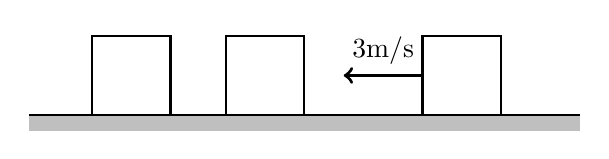
\begin{tikzpicture}
        \fill[gray!50](0,0) rectangle(7,-.2);
        \begin{scope}[thick]
          \draw(0,0)--(7,0);
          \draw(.8,0) rectangle(1.8,1);
          \draw(2.5,0) rectangle(3.5,1);
          \draw(5,0) rectangle(6,1);
        \end{scope}
        \draw[very thick,->](5,.5)--(4,.5) node[midway,above]{\SI{3}{m/s}};
      \end{tikzpicture}
    \end{center}
  }
  
  \question The speed of the second mass after the collision is
    \label{3masses1}
    \begin{choices}
    \choice zero
    \choice\SI{1.5}{\metre\per\second}
    \choice\SI{3.}{\metre\per\second}
    \choice\SI{6.}{\metre\per\second}
    \choice\SI{9.}{\metre\per\second}
    \end{choices}

  \question The speed of the second and third masses after they collide
  inelastically is
  \label{3masses2}
  \begin{choices}
    \choice zero
    \choice\SI{1.5}{\metre\per\second}
    \choice\SI{3.0}{\metre\per\second}
    \choice\SI{6.0}{\metre\per\second}
    \choice\SI{9.0}{\metre\per\second}
  \end{choices}
  
  \uplevel{
    \textbf{Questions \ref{boy1}--\ref{boy2}}. A \SI{20}{\kilo\gram} boy runs
    at a speed of \SI{3}{\metre\per\second} and jumps onto a
    \SI{40}{\kilo\gram} sled on frictionless ice that is initially at rest. The
    boy and the sled then  move together for a short time.
  }

  \question The speed of the boy and sled after he jumps on it is
  \label{boy1}
  \begin{choices}
    \choice\SI{.5}{\metre\per\second}
    \choice\SI{.8}{\metre\per\second}
    \choice\SI{1.}{\metre\per\second}
    \choice\SI{1.5}{\metre\per\second}
    \choice\SI{2.}{\metre\per\second}
  \end{choices}
    
  \question While the boy and sled are moving, he jumps off the back of the
  sled in such a way the boy is at rest, and the sled continues to move forward.
  The speed of the sled after the boy jumps off is
  \label{boy2}
  \begin{choices}
    \choice\SI{1.5}{\metre\per\second}
    \choice\SI{2.}{\metre\per\second}
    \choice\SI{3.}{\metre\per\second}
    \choice\SI{4.5}{\metre\per\second}
    \choice\SI{6.}{\metre\per\second}
  \end{choices}
    
  \question A 1.0 kg block is released from rest from a height $h$ at the top
  of a fixed curved ramp of negligible friction. The block slides down the ramp
  and collides with another block of mass 1.5 kg at rest at the bottom of the
  ramp. The two blocks stick together and move with a speed of
  \SI5{\metre\per\second}. The height $h$ from which the 1.0 kg block began is
  \begin{choices}
    \choice 0.8 m
    \choice 1.2 m
    \choice 1.8 m
    \choice 2.8 m
    \choice 7.8 m
  \end{choices}
  \newpage
  
  \question A dart of mass $m$ is fired into a wooden block of mass $4m$ that
  hangs from a string. The dart and block then rise to a maximum height $h$. An
  expression for the initial speed $v_0$ of the dart before striking the block
  is
  \begin{choices}
    \choice$\sqrt{gh}$
    \choice$\sqrt{2gh}$
    \choice$\sqrt{50gh}$
    \choice$\sqrt{100gh}$
    \choice$\sqrt{250gh}$
  \end{choices}

  \question A mass $m_1$ initially moving at speed $v_0$ collides with and
  sticks to a spring attached to a second, initially stationary mass $m_2$. The
  two masses continue to move to the right on a frictionless surface as the
  length of the spring oscillates. At the instant that the spring is maximally
  extended, the velocity of the first mass is
  \begin{center}
    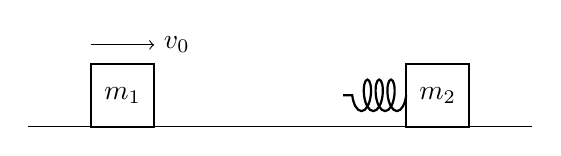
\begin{tikzpicture}[scale=.8]
      \draw[->](1,1.3)--(2,1.3) node[right]{$v_0$};
      \draw(0,0)--(8,0);
        \draw[thick](1,0) rectangle (2,1) node[midway]{$m_1$};
        \draw[thick](6,0) rectangle (7,1) node[midway]{$m_2$};
        \draw[thick,
          decoration={aspect=.4,segment length=1.5mm, amplitude=2mm,coil},
          decorate] (6,.5)--(5,.5);
    \end{tikzpicture}
  \end{center}
  \begin{choices}
    \choice $v_0$
    \choice $m_1^2v_0/(m_1+m_2)^2$
    \choice $m_2v_0/m_1$
    \choice $m_1v_0/m_2$
    \choice $m_1v_0/(m_1+m_2)$
  \end{choices}

  \question Two masses moving along the coordinates axes as shown collide at the
  origin and stick to each other. What is the angle $\theta$ that the final
  velocity that makes with the $x$-axis?
  
  \begin{minipage}{.4\linewidth}
    \begin{tikzpicture}[scale=.7]
      \draw(-4,0)--(4,0);
      \draw(0,-3)--(0,3);
      \draw[very thick,->](-3,0)--(-1,0)node[midway,below]{\small$\bm{v}_1$};
      \draw[very thick,->](0,-2)--(0,-1) node[midway,right]{\small$\bm{v}_2$};
      \draw[very thick,->](0,0)--(1.3,1.3)node[right]{\small$\bm{v}_f$};
      \draw[fill=gray](-3,0) circle(.2) node[above]{\small$m_1$};
      \draw[fill=gray](0,-2) circle(.2) node[right]{\small$m_2$};
      \draw[<->] (.75,0) arc(0:45:.75) node[pos=.6,right]{\small$\theta$};
    \end{tikzpicture}
  \end{minipage}
  \begin{minipage}{.5\linewidth}
    \begin{choices}
      \choice $\tan^{-1}(v_2/v_1)$
      \choice $\tan^{-1}[m_1v_1/(m_1+m_2)]$
      \choice $\tan^{-1}(m_1v_2/m_2v_1)$
      \choice $\tan^{-1}(m_2v_2^2/m_1v_1^1)$
      \choice $\tan^{-1}(m_2v_2/m_1v_1)$
    \end{choices}
  \end{minipage}

  \question A mass traveling in the $+x$ direction collides with a mass at rest.
  Which of the following statements is true?
  \begin{choices}
    \choice After the collision, the two masses will move with parallel
    velocities
    \choice After the collision, the masses will move with anti-parallel
    velocities
    \choice After the collision, the masses will both move along the $x$-axis
    \choice After the collision, the $y$-components of the velocities of the two
    particles will sum to zero.
    \choice None of the above
  \end{choices}
  \newpage

  % TAKEN FROM THE 2016 AP PHYSICS 1 EXAM FREE-RESPONSE QUESTION #2
  \question A new kind of toy ball is advertised to ``bounce perfectly
  elastically'' off hard surfaces. A student suspects, however, that no
  collision can be perfectly elastic. The student hypothesizes that the
  collisions are very close to being perfectly elastic for low-speed collisions
  but that they deviate more and more from being perfectly elastic as the
  collision speed increases.
  \begin{parts}
    \part Design an experiment to test the student's hypothesis about collisions
    of the ball with a hard surface. The student has equipment that would
    usually be found in a school physics laboratory.
    \begin{subparts}
      \subpart What quantities would be measured?
      
      \subpart What equipment would be used for the measurements, and how would
      that equipment be used?
      
      \subpart Describe the procedure to be used to test the student's
      hypothesis. Give enough detail so that another student could replicate
      the experiment.
    \end{subparts}
    \part Describe how you would represent the data in a graph or table. Explain
    how that representation would be used to determine whether the data are
    consistent with the student's hypothesis.
    
    \part A student carries out the experiment and analysis described in parts
    (a) and (b). The student immediately concludes that something went wrong in
    the experiment because the graph or table shows behavior that is elastic
    for low-speed collisions but appears to violate a basic physics principle
    for high-speed collisions.
    \begin{subparts}
      \subpart Give an example of a graph or table that indicates nearly elastic
      behavior for low-speed collisions but appears to violate a basic physics
      principle for high-speed collisions.
      
      \subpart State one physics principle that appears to be violated in the
      graph or table given in part (c)i. Several physics principles might
      appear to be violated, but you only need to identify one.

      \subpart Briefly explain what aspect of the graph or table indicates that
      the physics principle is violated, and why.
    \end{subparts}
  \end{parts}
  \newpage

  \uplevel{
    \cpic{.4}{ballastic}
  }
  \question The Ballistic Pendulum. To determine the muzzle speed of a gun, a
  bullet is shot into a mass $M$ from a string as shown below, causing $M$ to
  swing upward through a maximum angle of $\theta$.
  \begin{parts}
    \part What is the speed of $M$ the instant after the bullet lodges in it?
    \part What is the speed of the bullet before it hits $M$?
    \part What is the tension in the string at the highest point of the
    pendulum's swing (when the string makes an angle of $\theta$ with the
    vertical as shown)?
  \end{parts}
  \newpage
  
  \question An \SI{800}{\kilo\gram} car is traveling along a wet road at a
  velocity of \SI{25.5}{\metre\per\second}. A \num{1000.}-kg car is traveling
  along the same road in the same direction at \SI{34.7}{\metre\per\second}.
  The two cars collide and lock together. Answer the following questions.
  \begin{parts}
    \part The two interlocked cars proceed at what velocity after the collision?
    \part Compare the kinetic energy of the two-car system immediately before
    the collision and after the collision.
    \part Discuss any transfer of energy that occurs, and explain whether this
    is an elastic or inelastic collision.
    \part If the coefficient of sliding friction between the tires of the cars
    and the wet pavement is 0.7, calculate the force of friction.
    \part How long does it take for the two interlocked cars to come to a
    complete stop on the wet pavement?
  \end{parts}
  \newpage

  \uplevel{
    \cpic{.5}{balance}
  }
  
  \question A stream of glass beads, each with a mass of 0.5 g, comes out of a
  horizontal tube at 100 per second. The beads fall a distance of 0.5 m to a
  balance pan and bounce back to their original height as shown in the figure
  below. How much mass must be placed in the other pan of the balance to keep
  the pointer at zero?
  \newpage

  \uplevel{
    \centering
    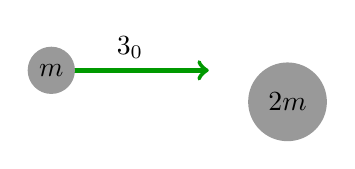
\begin{tikzpicture}
      \draw[ultra thick,green!60!black,->](0,0)--(2,0)
      node[midway,above,black]{$3\varv_0$};
      \fill[gray!80](0,0) circle(.3) node[black]{$m$};
      \fill[gray!80](3,-.4) circle(.5) node[black]{$2m$};
    \end{tikzpicture}
    \hspace{1in}
    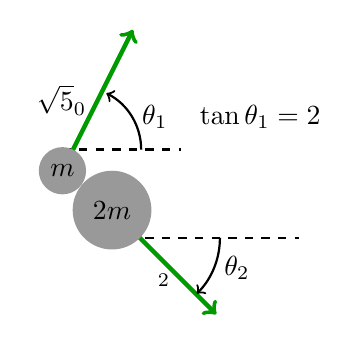
\begin{tikzpicture}
      \draw[ultra thick,green!60!black,->,rotate=atan(2)](0,0)--(2,0)
      node[midway,left,black]{$\sqrt5\varv_0$};
      \draw[thick,dashed](0,{.3*sin(atan(2))})--(1.5,{.3*sin(atan(2))});
      \draw[thick,->](1,{.3*sin(atan(2))}) arc(0:atan(2):.8)
      node[midway,right]{$\theta_1\quad\tan\theta_1=2$};
      \fill[gray!80](0,0) circle(.3) node[black]{$m$};
      \draw[
        ultra thick,
        green!60!black,->,
        rotate around={-atan(1):(.63,-.5)}](.63,-.5)--(2.5,-.5)
      node[midway,below,black]{$\varv_2$};
      \draw[thick,dashed](.63,{-.5-.5*sin(atan(1))})--(3,{-.5-.5*sin(atan(1))});
      \fill[gray!80](.63,-.5) circle(.5) node[black]{$2m$};
      \draw[thick,->](2,{-.5-.5*sin(atan(1))}) arc(0:-atan(1):1)
      node[midway,right]{$\theta_2$};
    \end{tikzpicture}
  }
  \question The figure above shows the results of a collision of two objects of
  unequal mass.
  \begin{parts}
    \part Find the speed of $v_2$ and angle $\theta_2$ of the larger mas after
    the collision.
    \part Show that the collision is elastic.
  \end{parts}
\end{questions}
\end{document}
